\documentclass{article}
\usepackage{float}
\usepackage{amsmath}
\usepackage{hyperref}
\usepackage{enumerate}
\usepackage{graphicx}
\graphicspath{ {./images/} }
\usepackage[style=authoryear]{biblatex}
\addbibresource{citations.bib}

\title{Machine Learning Engineer Nanodegree \\
\large Capstone Project}
\author{Haitham Alhad Hyder}

\begin{document}

\maketitle

\section{Definition}\label{definition}

Note:\emph{(approx. 1-2 pages)}

\subsection*{Project Overview}\label{project-overview}

The project involves the infamous Titanic sinkage of 1912. The data set
and inspiration to solve the problem from the Titanic challenge
Kaggle competition \parencite{kaggle}.

Only 1502 of the 2224 on board the ship survived and was a big tragedy
since it was labelled the ``unsinkable'' ship. We will be building a
model that will identify the chance of survival a person has.

\subsection{Problem Statement}\label{problem-statement}

We will be building a model that inputs the characteristics of a person
and outputs a value between 0 and 1 giving us the chance of someone
surviving.

The model that we come up with should be capable of identifying patterns
that affect the chance of survival and therefore, by rounding the
probability it outputs we can tell if that person's prediction is
survival or not.

The steps to solving this problem are as follows:

\begin{enumerate}
\item
  Loading up the train data and split it into a train, validation and
  test data sets.
\item
  Build an XGBoost binary linear classifier as well as a PyTorch neural
  network.
\item
  At the same time we build an SKLearn decision tree which will be our
  Statistical base model that will help us compare it to our ML(Machine
  Learning) models.
\item
  After evaluating all the models and picking the best one, we will
  deploy to an API endpoint.
\item
  Finally we will create a web page that communicates with our model;
  sending in a user's chosen passenger characteristics and outputting
  the probability of survival.
\end{enumerate}

\subsection{Metrics}\label{metrics}

The main criteria that would help us evaluate the models we create is
accuracy.

\[ 
  \text{accuracy $=\frac{\text{true positive} + \text{true negative}}{\text{dataset size}}$}
\]

Since we are not extremely concerned with neither false negatives nor false positives,
using accuracy as the chosen metric is much better than recall or precision.
We only want to know out of the total inputs what percentage of them did we label correctly.

\section{Analysis}

Note: \emph{(approx. 2-4 pages)}

\subsection{Data Exploration}\label{data-exploration}

The train csv file which is the only one we will use since the test csv file, doesn't
contain labels making it useless in evaluating our models. It contains data on 891
passengers.

\begin{table} [H]
    \begin{tabular}{ ||p{2cm}||p{6cm}|p{2.5cm}||  }
        \hline
        \multicolumn{3}{|c|}{\textbf{Data columns}} \\
        \hline
        \textbf{Variable} & \textbf{Definition} & \textbf{Key} \\
        \hline\hline
        \textbf{Survived} & \emph{Label} if a person survived or not & $0$ = No; $1$ = Yes \\ 
        \hline \hline
        \textbf{Pclass} & 
            Ticket class
            \newline
            \emph{Proxy for  socioeconomic status (SES)} &
            1 = 1st (upper), 
            \newline 2 = 2nd (middle), 
            \newline 3 = 3rd (lower) \\
        \hline
        \textbf{Sex} & The gender of the person & {} \\ 
        \hline
        \textbf{Age} & The age in years & {} \\ 
        \hline
        \textbf{SibSp} &
            \# of siblings and spouses aboard
            \newline
            \newline
            \emph{Note:} 
            Sibling = (brother, sister, stepbrother, stepsister)
            \newline
            Spouse = (husband, wife)
            & {} \\ 
        \hline
        \textbf{Parch} & 
            \# Parents and children aboard
            \newline
            \newline
            \emph{Note:} 
            Parent = (mother, father)
            \newline
            Child = (daughter, son, stepdaughter, stepson)
            & {} \\ 
        \hline
        \textbf{Fare} & Passenger fare & {} \\ 
        \hline
        Embarked & Port of embarkation & 
            C = Cherbourg,
            \newline Q = Queenstown, 
            \newline S = Southampton \\ 
        \hline
        PassengerId  & A unique number for each person &  \\
        \hline
        Name & The Name of the passenger & {} \\
        \hline
        Ticket & The unique ticket number & {} \\ 
        \hline
        Cabin & Cabin number & {} \\ 
        \hline
   \end{tabular}
   \caption{\label{tab:data-columns}The variables within the data set}
\end{table}

The columns that are not bolded have various problems such as having many 
null values (e.g. Cabin) or not being relevant in solving the problem
(e.g. PassengerId) and will not be used to build the features of the models.

\begin{table} [H]
    \begin{tabular}{lrrrrrr}
        \hline
        {} &     Survived &      Pclass &         Age &       SibSp &       Parch &        Fare \\
        \hline
        count &   891.000000 &  891.000000 &  714.000000 &  891.000000 &  891.000000 &  891.000000 \\
        mean  &    0.383838 &    2.308642 &   29.699118 &    0.523008 &    0.381594 &   32.204208 \\
        std   &    0.486592 &    0.836071 &   14.526497 &    1.102743 &    0.806057 &   49.693429 \\
        min   &    0.000000 &    1.000000 &    0.420000 &    0.000000 &    0.000000 &    0.000000 \\
        25\%  &    0.000000 &    2.000000 &   20.125000 &    0.000000 &    0.000000 &    7.910400 \\
        50\%  &    0.000000 &    3.000000 &   28.000000 &    0.000000 &    0.000000 &   14.454200 \\
        75\%  &    1.000000 &    3.000000 &   38.000000 &    1.000000 &    0.000000 &   31.000000 \\
        max   &    1.000000 &    3.000000 &   80.000000 &    8.000000 &    6.000000 &  512.329200 \\
        \hline
    \end{tabular}
    \caption{\label{tab:data-stats}Statistics of the data before cleaning and processing}
\end{table}

Table \ref{tab:data-stats} gives us interesting insights into the data. The mean of survived
tells us that most people among the 891 didn't survive. Since the mean is much closer
to 0 while the median is at 0.

The average age of the passengers we have is around 30 years old.

\subsection{Exploratory
Visualization}\label{exploratory-visualization}

To visualize the data we first have to clean the data set as discussed in \ref{data-preprocessing}.

\begin{figure}[H]
    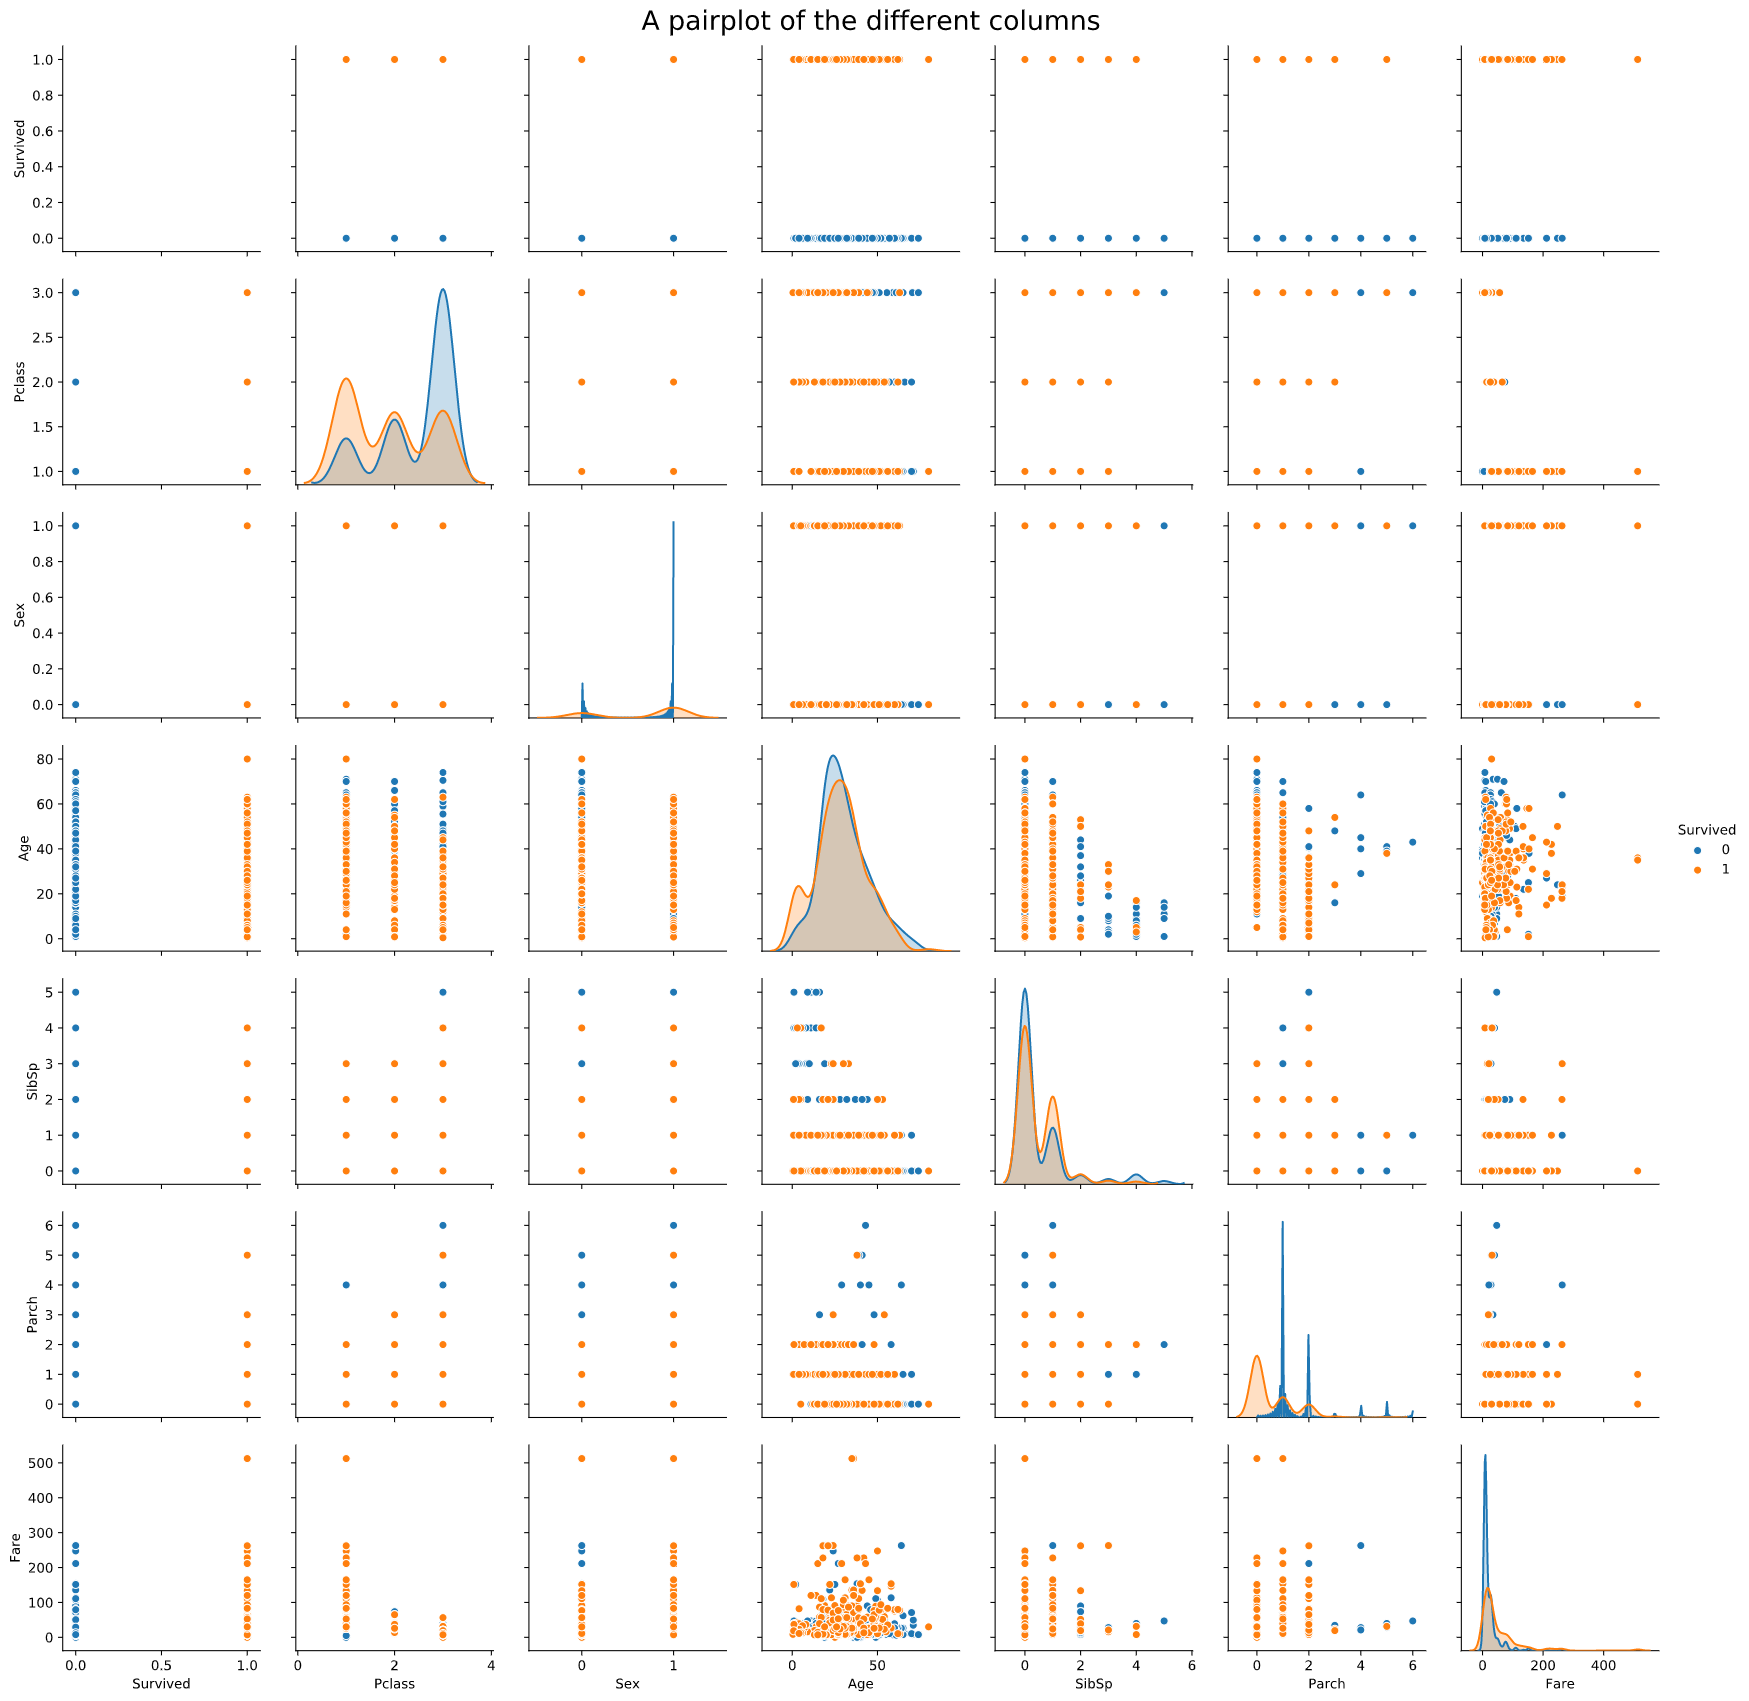
\includegraphics[width=\linewidth]{pairplot}
    \caption{A pair plot of the cleaned columns that helps us to start identifying patterns
    of features that might increase chances of survival}
    \label{fig: pair-plot}
\end{figure}

The figure \ref{fig: pair-plot} plot suggests that the lower \emph{Pchar} value a person has, 
the higher their chances of survival.

\subsection{Algorithms and
Techniques}\label{algorithms-and-techniques}

The modelling algorithms that we use are: sci-kit learn decision tree, XGBoost binary classifier,
and a PyTorch Neural Network.

All the following models take in the 6 inputs we identified in table \ref{tab:data-columns}.

The decision tree identifies how the data is segmented leading to a specific label (0 or 1 [Survived]).
We will use the default values parameters except max\_depth that we set to 10.

The XGBoost algorithm builds a logistic function model that gives us the probability between 0 and 1.
All the hyper-parameters were left at their default values except the following:

\begin{itemize}
    \item 
        max\_depth=10 [matching it to that of the decision tree]
    \item 
        eta=0.2
    \item 
        gamma=4
    \item 
        min\_child\_weight=6
    \item 
        subsample=0.8
    \item 
        silent=0
    \item 
        objective='binary:logistic'
    \item 
        early\_stopping\_rounds=10
    \item 
        num\_round=500
\end{itemize}

While the PyTorch model produces a single output that is also a value 0 or 1 and the following 
hyper-parameters:

\begin{itemize}
    \item "input\_features": 6
    \item "hidden\_dim": 30
    \item "output\_dim": 1
    \item "epochs": 250
\end{itemize}

\subsection{Benchmark}\label{benchmark}

The manner that we evaluate the different values is using the accuracy of the multiple models.
The Sci-kit learn which is our base model, has an 80\% accuracy. Therefore, the goal was to get
an accuracy higher than 80\%.

\section{Methodology}\label{methodology}

Note: \emph{(approx. 3-5 pages)}

\subsection{Data Preprocessing}\label{data-preprocessing}

For processing we begin by cleaning the data then splitting it into training, validation and test data sets.
To clean the data we:
\begin{enumerate}
    \item first, map the gender values to the following: male = 0, female = 1.
    \item then, only pick the columns (the bolded variables in table \ref{tab:data-columns}) we require
    \item and finally drop all the rows with null values.
\end{enumerate}

During inference using the web app, we prevent users from submitting data for inference,
unless it is correct and contains only the variables we require.

\subsection{Implementation}\label{implementation}

In this section, we first had to train the models, then creating the web app and API endpoint.

The sci-kit learn Decision Tree is just a statistical model that doesn't require training.

To Train the XGBoost model, we fit training data and optimize on 
reducing the validation error rate.

For the PyTorch model, which has the following architecture:
\begin{itemize}
    \item Fully connected layer taking in the 6 inputs
    \item Passing it to the 30 hidden Fully connected Layers
    \item And outputting a single a value
\end{itemize}
The loss function that we use is the BCELoss and we use the Adam optimizer.

An important update that occurred after implementing the solutions, was
that only the XGBoost model produces a probability while the other two models 
produce a binary value representing survival.

During the application development cycle, we first had to deploy the chosen model,
then create a lambda function that invokes the model and finally create an API gateway
that will allow us to send and receive data from our lambda function.

A complication that occurred was that the lambda function has to carry out 
extra computations to save the user's input into a .npy file then send that 
to our model for inference.

\subsection{Refinement}\label{refinement}

Firstly, we used the sci-kit learn model that had an accuracy of 80\%,
next, we made a new model, this time being an XgBoost model that yielded 
and 81\% accuracy which is not a great leap forward.

Therefore, going the extra mile and using a neural network in the hopes of it
learning the different patterns involved within the data set might yield a higher
accuracy and it did. The PyTorch model test set accuracy was 85\%.

To improve our already great model, one option was reducing the model complexity
and using 20 instead of 30 hidden layers. The accuracy drops to 84\% however, 
recall increases from 70\% to 72\%. Since we mentioned that recall and precision
do not matter as much as accuracy, we stick with our first PyTorch model as the best
model so far.

In this section, you will need to discuss the process of improvement you
made upon the algorithms and techniques you used in your implementation.
For example, adjusting parameters for certain models to acquire improved
solutions would fall under the refinement category. Your initial and
final solutions should be reported, as well as any significant
intermediate results as necessary. Questions to ask yourself when
writing this section:

\subsection{Results}\label{kaggleresults}

Note: \emph{(approx. 2-3 pages)}

\subsection{Model Evaluation and
Validation}\label{model-evaluation-and-validation}

In this section, the final model and any supporting qualities should be
evaluated in detail. It should be clear how the final model was derived
and why this model was chosen. In addition, some type of analysis should
be used to validate the robustness of this model and its solution, such
as manipulating the input data or environment to see how the model's
solution is affected (this is called sensitivity analysis). Questions to
ask yourself when writing this section:

\begin{itemize}
\item
  \emph{Is the final model reasonable and aligning with solution
  expectations? Are the final parameters of the model appropriate?}
\item
  \emph{Has the final model been tested with various inputs to evaluate
  whether the model generalizes well to unseen data?}
\item
  \emph{Is the model robust enough for the problem? Do small
  perturbations (changes) in training data or the input space greatly
  affect the results?}
\item
  \emph{Can results found from the model be trusted?}
\end{itemize}

\subsection{Justification}\label{justification}

The final model is a PyTorch Neural Network trained with the
hyper-parameters described in section \ref{algorithms-and-techniques}.

The results we found with this model are much stronger than the benchmark
result and therefore, is a much better model to use. It does a much better
job in labelling a person as survived or not.

\begin{center}
    \begin{table}[h]
        \begin{tabular}{lrrrr}
            \hline
            {} &     SKLearn &     XGBoost  &         PyTorch (30) &  PyTorch (20) \\
            \hline
            precision &     0.712 &     0.926 &     0.854 &     0.818  \\
            recall    &     0.740 &     0.500 &     0.700 &     0.720  \\
            \hline
            Accuracy  &     0.804 &     0.811 &   \textbf{0.853} &    0.846  \\
            \hline
        \end{tabular}
        \caption{\label{tab:data-results}The evaluation metrics of the different models 
            \emph{The 30 and 20 represent the number of hidden layers}}
    \end{table}
\end{center}

\section{Conclusion}\label{conclusion}

Note: \emph{(approx. 1-2 pages)}


\subsection{Free-Form Visualization}\label{free-form-visualization}

\begin{figure}[H]
    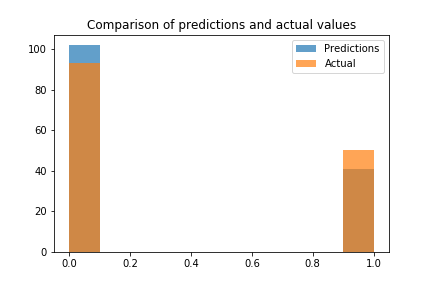
\includegraphics[width=\linewidth]{free-form}
    \caption{A comparison of the histograms of labels produced as predictions compared to 
        the actual labels of the test data set. It shows that the predicted values exaggerates
        the chances of someone not surviving and fails to label those who survive as survivors}
    \label{fig: free-form-plot}
\end{figure}

\begin{figure}[H]
    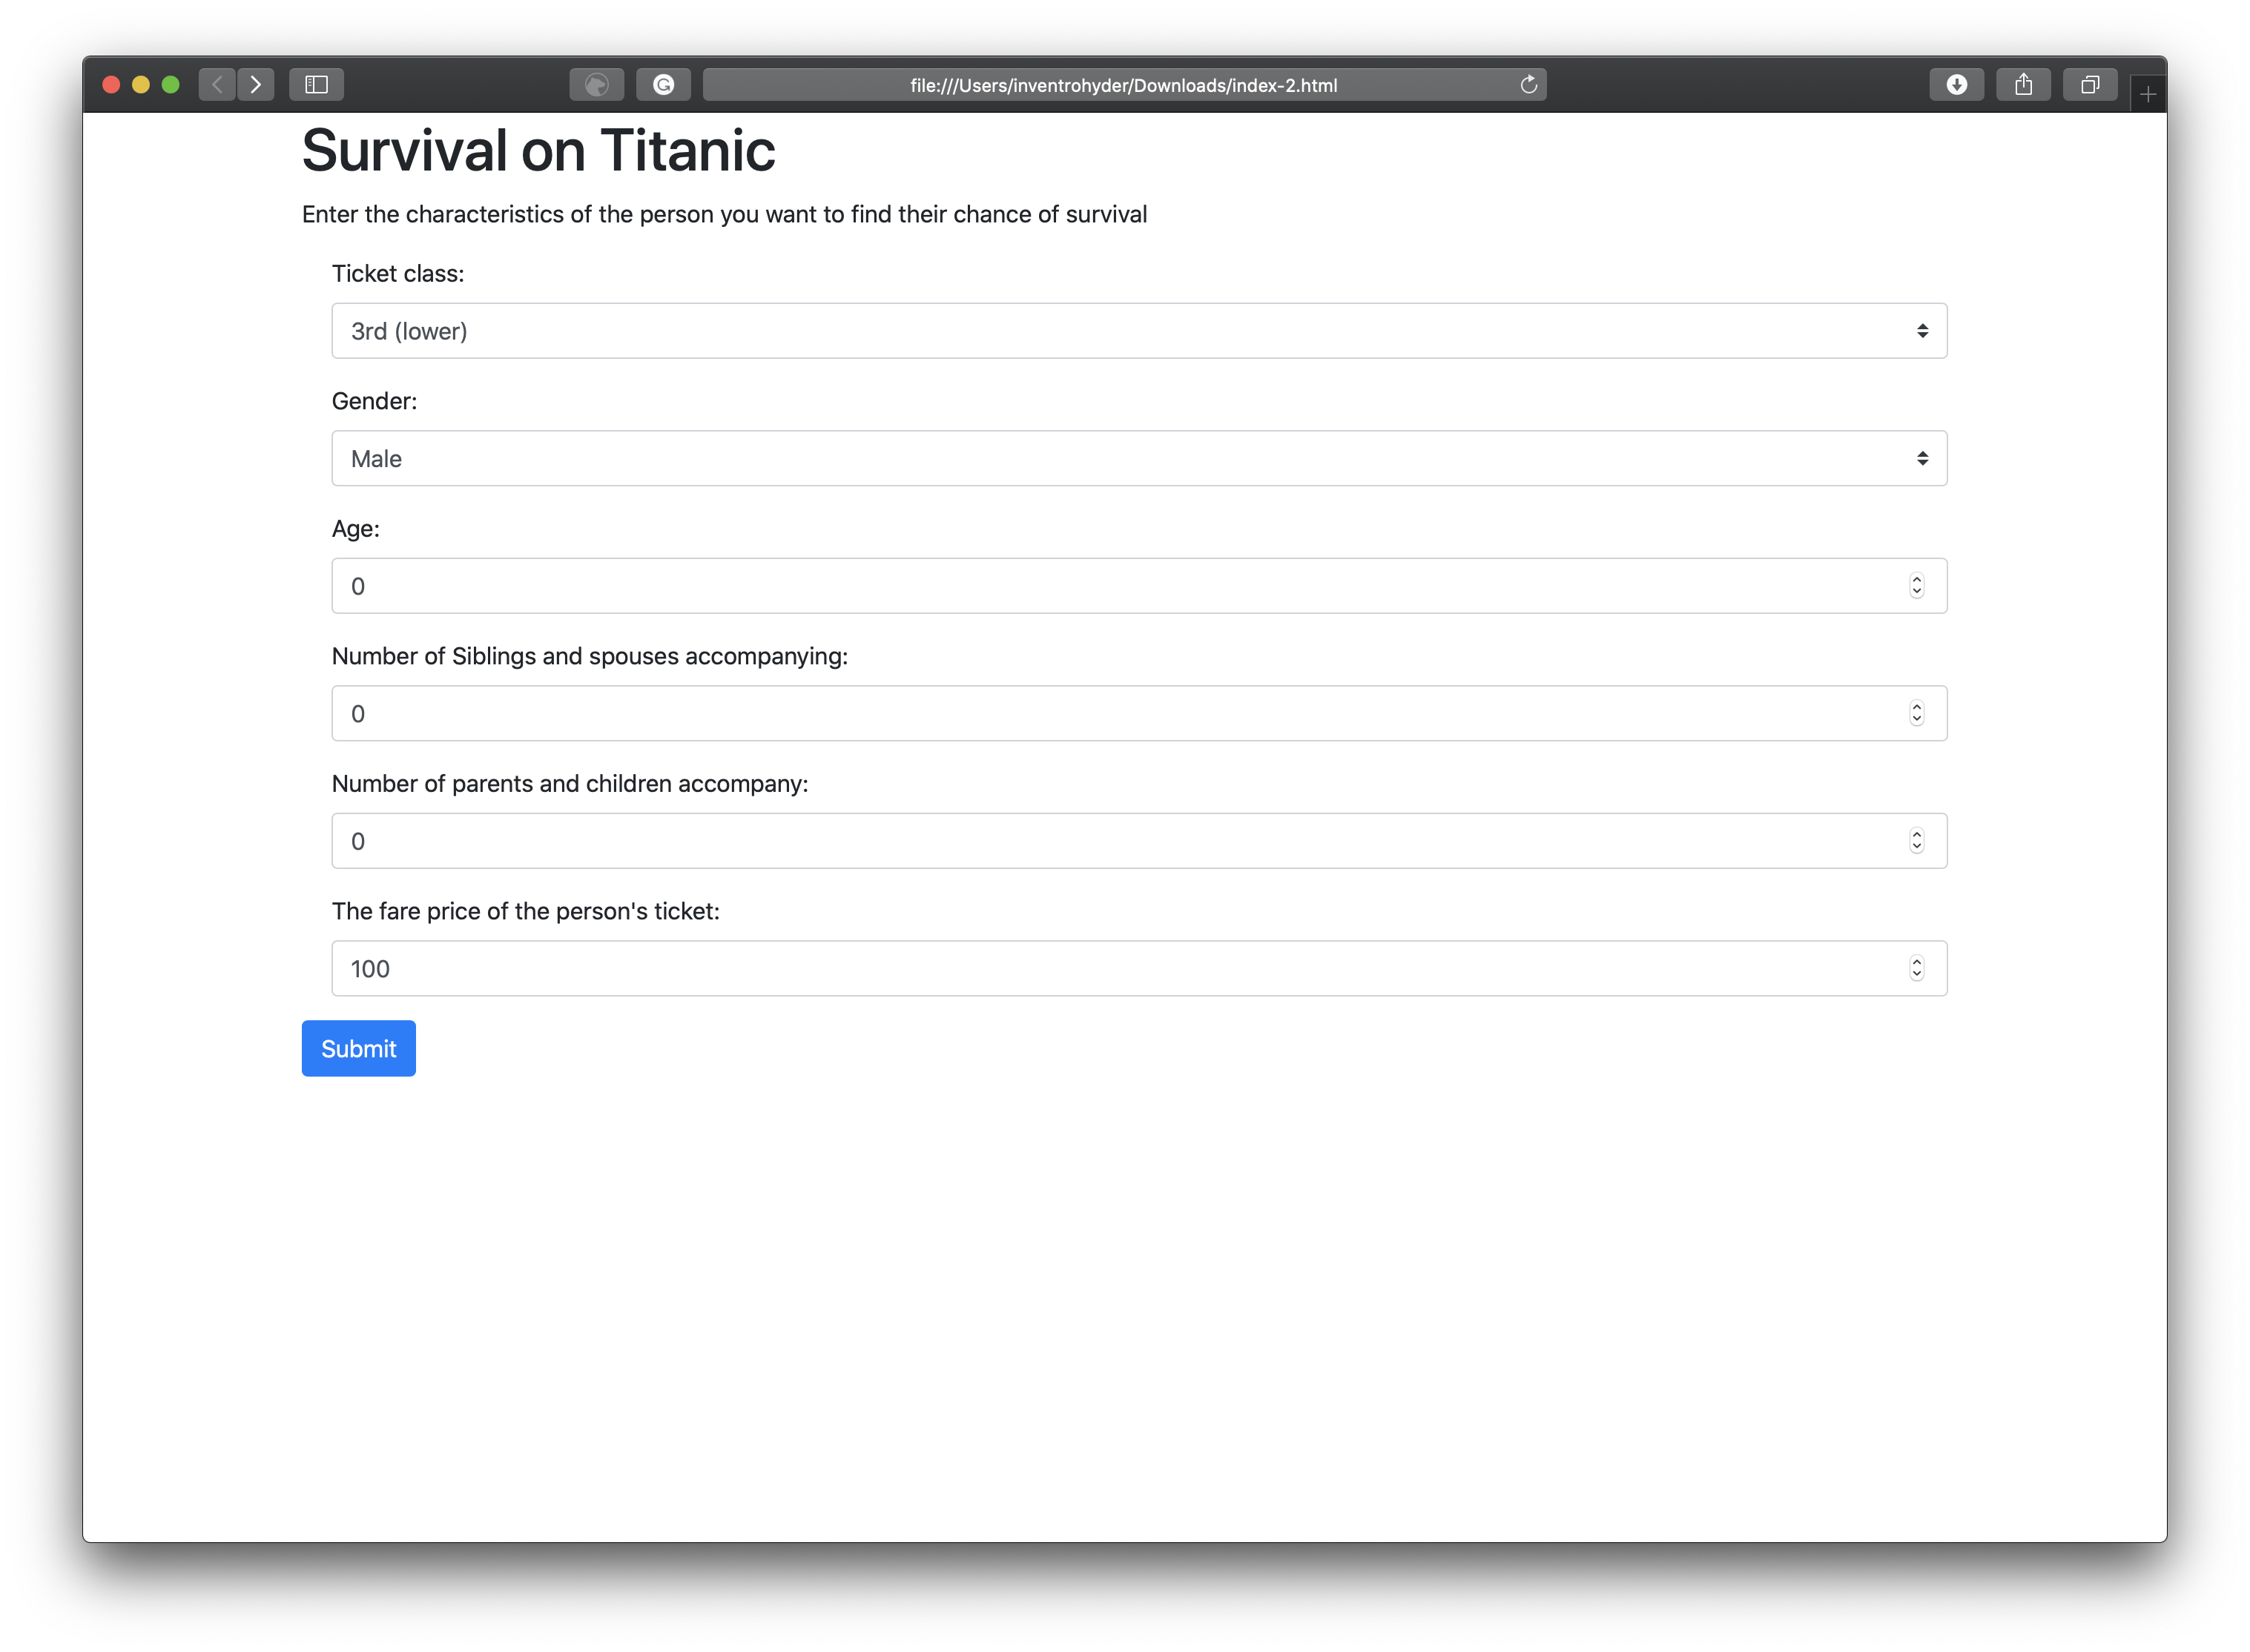
\includegraphics[width=\linewidth]{web_app}
    \caption{The web app that I made in-order to connect users with our deployed model.}
    \label{fig: free-form-plot}
\end{figure}

\begin{figure}[H]
    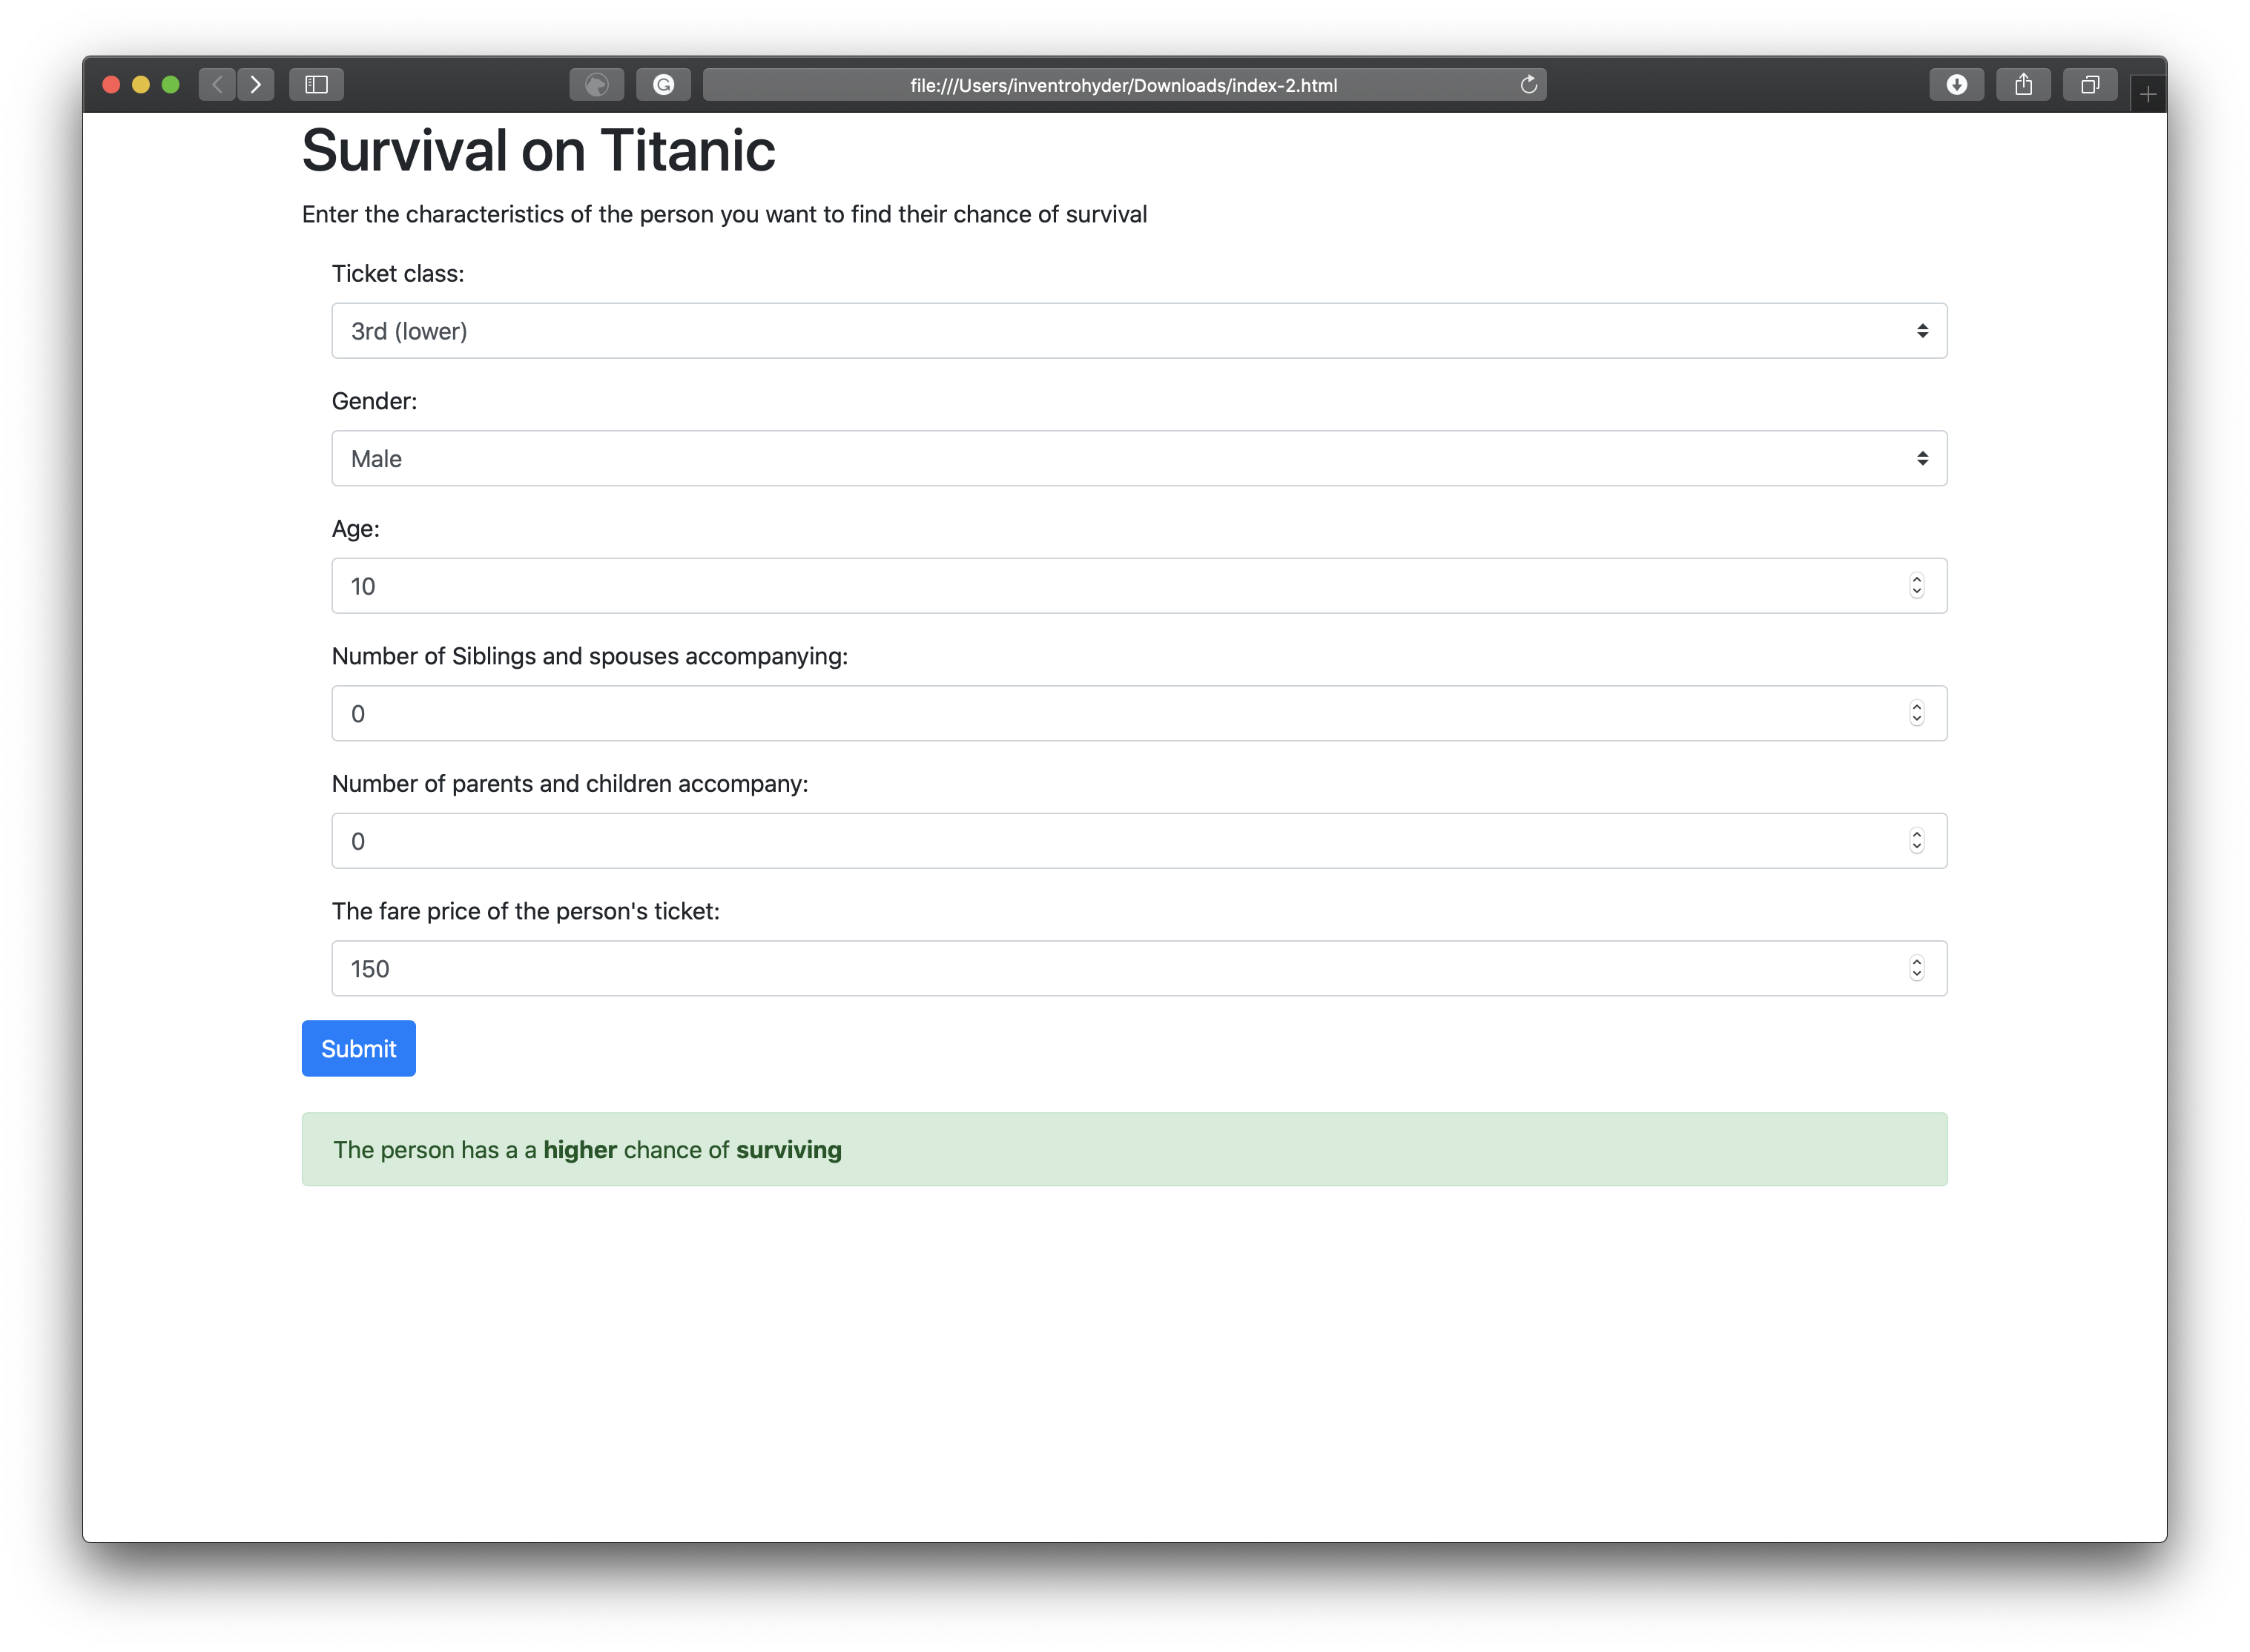
\includegraphics[width=\linewidth]{web_app_survive}
    \caption{An example of a predicted survival}
    \label{fig: free-form-plot}
\end{figure}

\begin{figure}[H]
    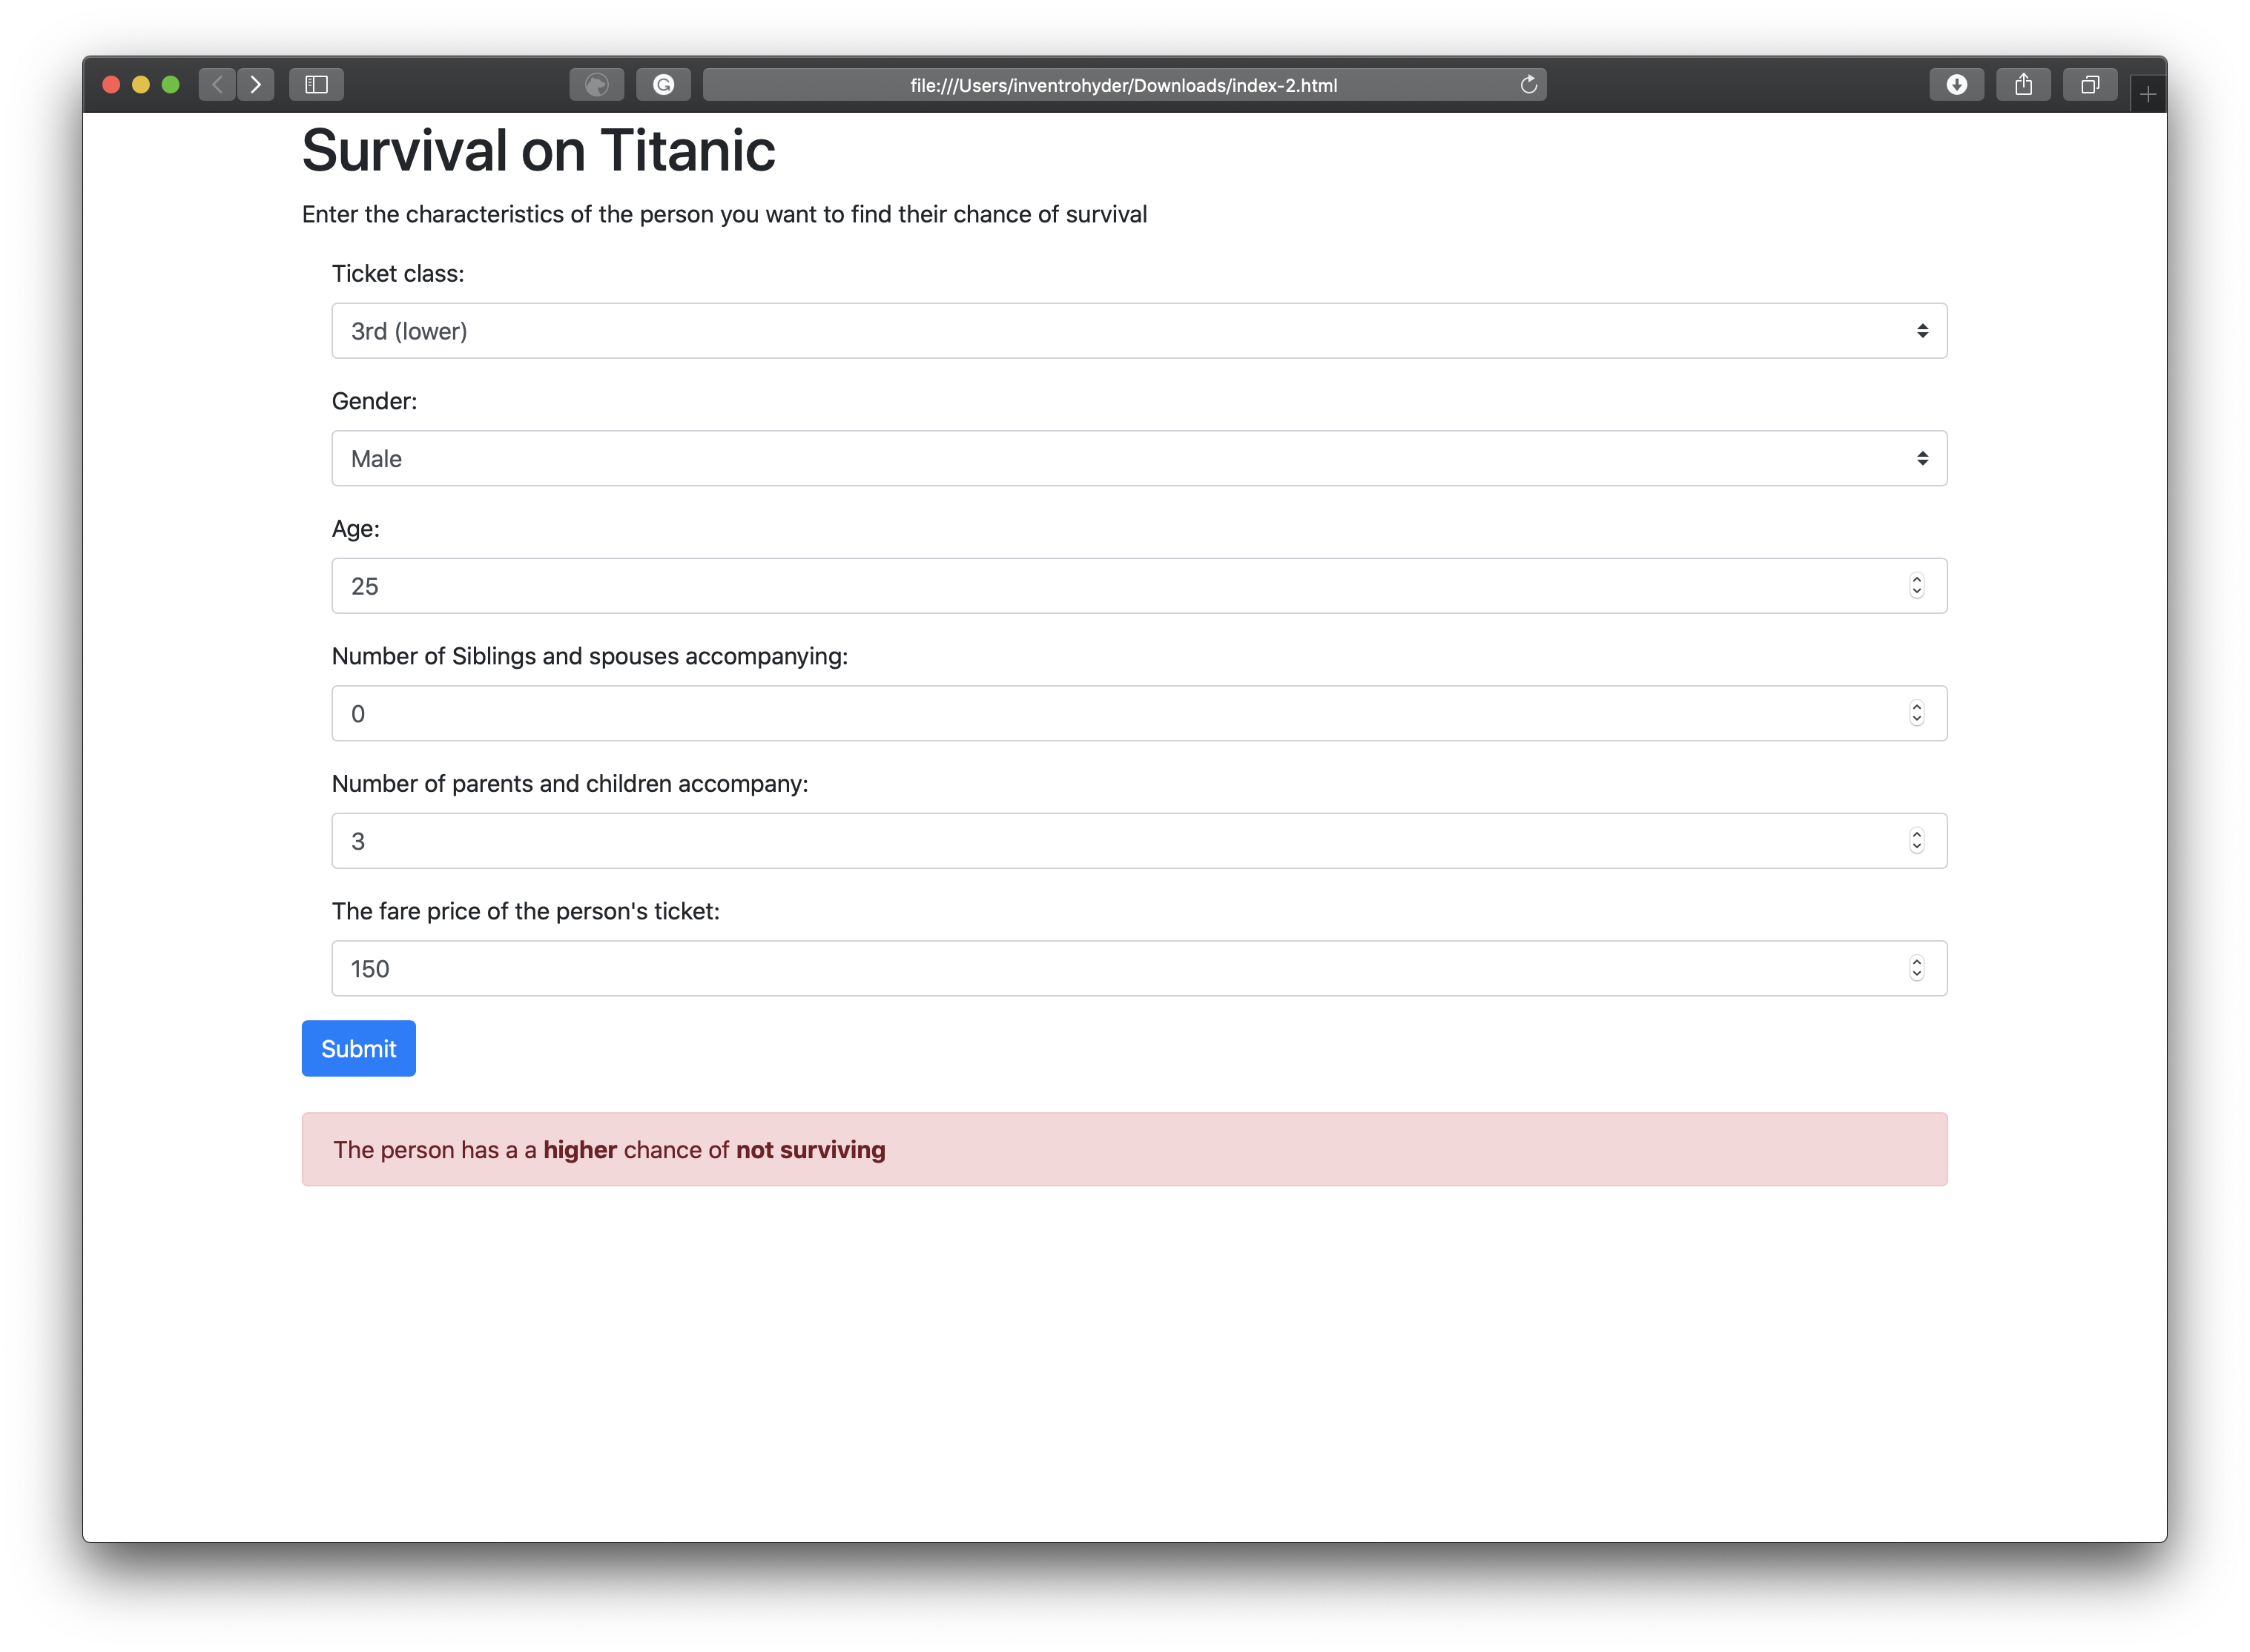
\includegraphics[width=\linewidth]{web_app_not_survive}
    \caption{An example of a predicted non-survival}
    \label{fig: free-form-plot}
\end{figure}

\subsection{Reflection}\label{reflection}

We can summarize the project as follows:
\begin{enumerate}
    \item Obtaining the data set and understanding the problem
    \item Cleaning the data and processing to pick out the features to use
    \item Choosing a modelling algorithm and fitting it (training)
    \item Comparing the different models using a metric to pick a better one
    \item Using the chosen model to make inferences for a web app
\end{enumerate}

One the key challenges that I got was trying to solve the errors that
occurred during the entire process and getting much more familiar with
cloud watch logs.

I also learnt that I can save Numpy arrays into .npy files which I didn't
realize till now.

The final model and web app were able to work and based on the accuracy we got
it seems it is a suitable model for this application.

\subsection{Improvement}\label{improvement}

I think there are further improvements that I could have made. One of which
would be the use of Hyperparameter tuning training jobs so that I can optimize
my models even further.

I haven't studied Deep Learning yet and the concepts that I used in this project
were from the tip of the iceberg of an introduction given within the coursework.
Therefore, I would love to understand them more deeply and have total insight of
them.

If I used the best model we got so far as the new benchmark, I hypothesis that a 
much better solution does exist. First, through the hyper-parameter tuning jobs
mentioned before, as well as through feature engineering which I didn't make the
best use of.

\begin{center}\rule{0.5\linewidth}{\linethickness}\end{center}

\textbf{Before submitting, ask yourself. . .}

\begin{itemize}
\item
  Does the project report you've written follow a well-organized
  structure similar to that of the project template?
\item
  Is each section (particularly \textbf{Analysis} and
  \textbf{Methodology}) written in a clear, concise and specific
  fashion? Are there any ambiguous terms or phrases that need
  clarification?
\item
  Would the intended audience of your project be able to understand your
  analysis, methods, and results?
\item
  Have you properly proof-read your project report to assure there are
  minimal grammatical and spelling mistakes?
\item
  Are all the resources used for this project correctly cited and
  referenced?
\item
  Is the code that implements your solution easily readable and properly
  commented?
\item
  Does the code execute without error and produce results similar to
  those reported?
\end{itemize}

\newpage
\printbibliography

\end{document}